\documentclass[a4paper]{report}
\usepackage[brazil]{babel}
\usepackage{graphicx}
\usepackage{imakeidx}
\usepackage{lettrine}
\usepackage[notlof]{tocbibind}

\makeindex[columns=3, title=keywords, intoc]

\title{Verde e Brutall}
\author{el comodin - smvb}
\date{agosto 2017}

\renewcommand*\contentsname{idx} 

\begin{document}
 
\maketitle
 
\tableofcontents

\clearpage

\addcontentsline{toc}{section}{Agradecimentos}
\section*{Agradecimentos}

Esta obra n\~ao seria poss\'ivel sem meus pais, Diva e Louren\c{c}o que me deram educa\c{c}\~ao, motiva\c{c}\~ao e as condi\c{c}\~oes para materializar este ensaio.
Agrade\c{c}o tambem a artista Lara Coletti pela ilustra\c{c}\~ao da capa e a Keista Lindo pela revis\~ao das vers\~oes em Portugu\^es e Ingl\^es.

e em especial um imenso obrigado a Ana Lidia Pimentel pelo seu lindo relato de momentos que viveu com seu pai e nos brinda com um conteudo maravilhoso de uma conversa que tivemos.  



\clearpage

\addcontentsline{toc}{section}{Pref\'acio}
\section*{Pref\'acio}


O mundo n\~ao nos deve nada, ele j\'a estava aqui antes. "Mark Twain"

O universo n\~ao tem obriga\c{c}\~ao de fazer sentido pra voc\^e. "Neil deGrasse Tyson"



a natureza n\~ao \'e sutil
ela curte um alvoro\c{c}o! \footnote{ as 18:44, 19 mar 2021 Andre Balen } 


\clearpage


\addcontentsline{toc}{section}{o verso}
\section*{janela aberta}

\lettrine[findent=2pt]{\fbox{\textbf{E}}}{ }ssa \'e a saga\index{saga} de um encontro com a m\'aquina, escrita por um motorista, e narrada por um autom\'ovel 
fabricado no brasil, desenhado por uma garota \footnote{Ana Lidia Pimentel, com quem tive o prazer de conversar em meados de maio de 2021}, filha de um empresario carioca, que administrou a f\'abrica de
 implementos agricolas e ferroviarios em Entre Rios.

A saga brasilis da injambra e do espirito criativo\index{criativo} aliada a emo\c{c}\~ao

Diversas aventuras, que ao longo do tempo vivenciei, me deram a ideia de 
registrar as coisas mais interessantes, pois sei que daqui pra frente vai ser cada vez mais dif\'icil algu\'em vicenciar, por diversos motivos, a modernidade e complexidade gradual dos meios de transporte dispon\'iveis, a propria
natureza humana de querer sempre facilitar, abstrair e afastar-se ao m\'aximo possivel de saber como as coisas funcionam, da aventura do risco e do instinto\index{instinto}.

Pra mim, \'e isso que significa um autom\'ovel antigo, afastar um passo do materialismo, de querer sempre o carro do ano, da moda, da preocupa\c{c}\~ao natural de nossos dias
e aproximar do natural, do divertido, do instinto e de tudo que da gra\c{c}a a vida, a aventura, a emo\c{c}\~ao.

E n\~ao sou o \'unico que pensa assim, vide mujica, grande mestre do nosso tempo que nao me deixa mentir \dots

\'E disso que se trata esse livro, o prazer da vida contado por uma maquina de 6 cilindros\index{6 cilindros}, 4 rodas e um cora\c{c}\~ao.

Agrade\c{c}o a todos os amigos(as) que fizeram parte desta aventura, e desde j\'a dedico esta obra a todos voc\^es.

\clearpage

\addcontentsline{toc}{section}{descoberta}
\section*{A descoberta}
Nos anos 80, quando eu tinha meus 11 anos, havia uma santa matilde\index{santa matilde} branco perolada na minha cidade,
eu passava por ela algumas vezes, indo ou voltando da escola, sempre achei o carro mais bacana de todos\dots

\addcontentsline{toc}{figure}{o sm branco}
\begin{figure}[!htb]
\centering
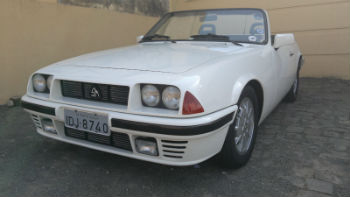
\includegraphics{sm_bco_per}
\caption{SM branco Perolado}
\label{sm_bco}
\end{figure}

Esta id\'eia fortaleceu na minha mente, quando em meados dos 80 o filme "devolta para o futuro" chegou aos cinemas, naturamente como todos nessa \'epoca
fui assistir e como amante de tecnologia e fic\c{c}\~ao fiquei encantado pra n\~ao dizer, abestado por aquele delorean, naturalmente a imagem da SM perolada
voltou para minha cabe\c{c}a como sendo o mais proximo que eu podia achar no brasil de uma. Salvo \'e claro os detalhes t\'ecnicos da viagem no tempo q requer
a lataria exposta para conduzir os 1.21 GigaWats pela superficie permitindo o deslocamento temporal \dots

Certo dia, pela manh\~a, seu Louren\c{c}o, meu falecido pai, me pediu para ligar o carro, um ford scort ghia, para aquecer o motor.

Mesmo n\~ao sendo necess\'ario para um carro relativamente moderno para \'epoca, para mim foi uma experi\^encia \'unica,
at\'e aquele momento, eu nunca havia ligado um carro, pra mim foi um divisor de \'aguas para a vida adulta.

Obviamente eu n\~ao fazia ideia do funcionamento da embreagem e da marcha, liguei o carro com a marcha engatada e por sorte
nao demoli a frente do carro, foi a unica e ultima vez que tive a chance de fazer aquilo, mas a emo\c{c}\~ao do motor ligando ficou
na minha mem\'oria. 

Naquele mesmo ano vi mais algumas vezes a SM branco perolado e pensei que se algum dia eu pudesse ter um
autom\'ovel, seria uma SM, esse dia chegou em 2011.
\clearpage
Eu estava visitando uns amigos em rio grande e fui convidado para almo\c{c}ar \`a bordo com a tripula\c{c}\~ao do Atl\~antico Sul.

\addcontentsline{toc}{figure}{atl\^antico Sul}
\begin{figure}[!htb]
\centering
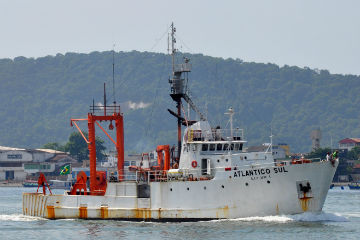
\includegraphics{atsul}
\caption{Navio oceanogr\'afico da FURG}
\label{at_sul}
\end{figure}

Durante o almo\c{c}o o assunto se dirigiu para autom\'oveis, lembrei do meu antigo sonho e compartilhei com o pessoal, nesta ocasi\~ao um dos marinheiros
me falou que havia uma santa matilde a venda em tapes, um conhecido.


Durante o almo\c{c}o o assunto se dirigiu para autom\'oveis, lembrei do meu antigo sonho e compartilhei com o pessoal, nesta ocasi\~ao um dos marinheiros
me falou que havia uma santa matilde a venda em tapes, um conhecido.

Durante o almo\c{c}o o assunto se dirigiu para autom\'oveis, lembrei do meu antigo sonho e compartilhei com o pessoal, nesta ocasi\~ao um dos marinheiros
me falou que havia uma santa matilde a venda em tapes, um conhecido.

Meu amigo Stefan, que havia convidado para o almo\c{c}o com sua equipe de trabalho, entusiamou-se com a informa\c{c}\~ao, e eu tambem, obviamente, e na semana 
seguinte fomos com mais um amigo de rio grande, Daniel Torres, vulgo "bala", outro entusiasta dos 6cilindros, ver a preciosidade.

Durante o trajeto, rio grande - tapes, conversamos muito, sobre os motores, a divers\~ao, pescarias, mas o que nao saia da cabe\c{c}a, a SM.   
\clearpage

\addcontentsline{toc}{section}{primeira vinda}

\section*{primeira vinda}

Era verde, assim como seu interior, perfeita, parecia tudo ok quando vimos, exceto os pneus, esses estavam na capa da gaita

\addcontentsline{toc}{figure}{273a sm}
\begin{figure}[!htb]
\centering
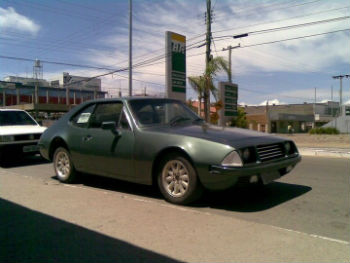
\includegraphics{sm273}
\caption{273$^{a}$SM fonte: Cadastro Nacional da Santa Matilde}
\label{a 273a SM}
\end{figure}
\clearpage


\addcontentsline{toc}{section}{4marchas (v)arretado}
\section*{4marchas (v)arretado}

Ela veio com cambio manual 4 marchas, \'e meu primeiro carro, adorei. Havia um click em cada marcha,
mais tarde num posto no cassino meu camarada Daniel torres me mostrou por que, o cambio era exposto!
Uma serie de alavancas mexiam diretamente nas engrenagens, essas dimensionadas pra nao faltar as demais 
marchas, a 3a era extremamente poderosa, e a quarta parecia ser mais leve que uma sexta, andava muito. 
Mas nao consegui aproveitar o suficiente eu acredito, passei uns 2 anos assim e percebi que o fato de 
acavalar as marchas deixava o auto pouco confi\'avel e optei por botar uma caixa de 5 marchas mais 
moderna.
Certamente foi a coisa que eu mais tenho saudade, acredito que todos que tiveram esta oportunidade 
se lembram dessa caixa de 4 marchas varetada.

\addcontentsline{toc}{figure}{4 marchas opala varetada}
\begin{figure}[!htb]
\centering
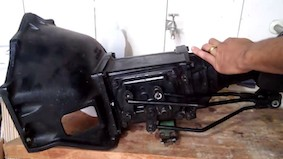
\includegraphics{caixa4}
\caption{caixa 4 marchas com click. fonte: google}
\label{4 marchas opala varetada}
\end{figure}
\clearpage


\addcontentsline{toc}{section}{Amaral Ferrador}
\section*{Amaral Ferrador}

Esse foi um acampamento que a matilde mostrou a que veio, fui encontrar uns amigos acampados durante
um feriado de NS.Navegantes na beira do rio, um lugar maravilhoso e eu nunca tinha ido.
Milagrosamente minha companheira da \'epoca aceitou o desafio, pegamos a estrada no meio da tarde e 
na estrada comecou uma chuva muito forte.
Estrada de chao, chuva forte, local que eu n\~ao conhecia, uma receita pra imprevistos mas n\~ao,
a sm nos levou seguros, encontrei o acampamento sem muito problema e os dias que seguiram foram muito bons
No domingo eu estava no meio do rio que era raso, eu sentado a agua batia no peito, vi ao longe se aproximar
a prociss\~ao que era composta por alguns barcos sendo o primeiro, o que carrega a imagem da santa.
Sai de onde eu estava pra n\~ao atrapalhar o movimento e logo que passaram voltei pro meu local para acompanhar.

Existem lugares fantasticos no interior do estado, um carro como a sm \'e perfeito para explora-los.


\addcontentsline{toc}{section}{reflex\~oes sobre o impacto ambiental}
\section*{reflex\~oes sobre o impacto ambiental}

Desde que me conheco por gente essa preocupac\~ao permeia a minha existencia, sou filho de biologos, e como tal
sempre procuro fazer essa reflex\~ao.
Estamos na era dos automoveis el\'etricos, e sou engenheiro eletricista, nada mais natural do que imaginar isso,
converter a santa matilde para el\'etrico. N\~ao farei este sacril\'egio, mas nao posso deixar de pensar nesta possibilidade.
Aqui na minha cidade existe uma empresa de motores e geradores, a weg, e outra empresa de colegas meus da puc, a fueltec, que
desenvolve sistemas de injecao mais eficientes e esta no momento fazendo kits de controle de torque para motores eletricos da weg
para automoveis como o fusca e o gol.
Existem prototipos maravilhosos, mas o custo obviamente eh bastante elevado.
Sobre o impacto, o simples fato de eu nao ter trocado de carro e ter adquirido uma sm usada ja me da bastante credito, apesar de
nao ter a eficiencia de um carro moderno. Entao neste quesito tenho a consciencia limpa, mas estou disponivel para argumentacao,
esta conversa me interessa bastante.



\addcontentsline{toc}{section}{fan clube}
\section*{fan clube}

Ao longo do tempo em que utilizei a santa matilde surgiram f\~ans um exemplo \'e este pessoal da unissinos, \footnote{http://www.budanga.com.br/2012/06/o-pessoal-hoje-eu-tava-chegando-no.html} 
Nesta mesma \'epoca um acontecimento inusitado colaborou para a iniciativa de escrever as aventuras.

\addcontentsline{toc}{figure}{inicio do fan clube}
\begin{figure}[!htb]
\centering
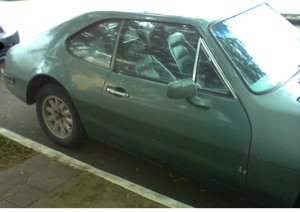
\includegraphics{Foto0296}
\caption{pessoal da unissinos fonte: www.budanga.com.br}
\label{fan clube SL }
\end{figure}


\addcontentsline{toc}{figure}{fan clube tecnosinos}
\begin{figure}[!htb]
\centering
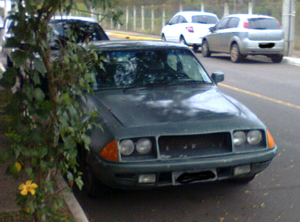
\includegraphics{Foto0295}
\caption{pessoal da unissinos fonte: www.budanga.com.br}
\label{Blog do pessoal da Tecnosinos }
\end{figure}
\clearpage

\addcontentsline{toc}{section}{o destino, eh o caminho, nocoes de proposito}


\section*{festivais}
	Muitos planos para os festivais, carros antigos lembram eventos mais tribais, e isso na verdade sao os festivais de hoje em dia, 
        estamos em outubro de 2019 proximo mes havera um festival no qual a verde e brutal conhece bem, ja trabalhou duro, caiu em valetas
        foi rebocada por fitas de e saiu mais feliz 

\section*{permacultura}
	Minha jornada com este naco de tecnologia formado por diversas ideias e solu\c{c}\~oes t\'ipicas de n\'os brasileiros\footnote{ a Snata matilde, feita de fibra de vidro, o mesmo material das pranchas de surf, tem mais de uma fun\c{c}\~ao, apesar de poluir de alguma forma segue um dos princ\'ipios da permacultura } me levou a conhecer a permacultura.
 	Me apaixonei, participei de diverosos mutir\~oes, reduzi o que pude todas as formas de pegada que eu pude deixando apenas plantas por onde passo, adoro plantar de tudo, de arvores a legumes,
        Conheci os principios da agricultura sintr\'opica e em dado momento pensei a rela\c{c}\~ao do ser humano com seus meios de transporte, passei a me concentrar muito em utilizar\footnote{e exercitar} meu corpo nos deslocamentos do dia a dia, mais saude menos combustivel f\'ossil, e passei a usar o autom\'ovel apenas para tarefas mais nobres como visitar amigos que moram longe, acampamentos e mutir\~oes.
	Esta escolha me trouxe sa\'ude e felicidade e recomendo a quem quiser se sentir mais leve. 


\section*{acampamentos}
	existe um vies filosofico no quesito acampamentos, este eh o proposito primordial no qual eu investi meu tempo para obter o dinheiro necessario para possuir uma maquina que me facilite esta atividade


\section*{pedra bacon}

 lembro q uma vez eu tava sentado dentro do rio viajando nas pedrinhas eu sentado a agua pela barriga, bem rasinho, mas no meio do rio
 achei uma pedra q parecia um cubinho de bacon  com as camadas umas de areia transparente outra mais fosca, bem um bacon fritinho
 levantei o olhar e vi uma aglomeraçao na beira do rio, um km adiante daonde eu tava
 ai eu fiquei bolado pensando qq ta rolando.  Dali a pouco olho pra tras e vem uns barcos pequenos, com um povo descendo o rio
 com a imagem da santa, era feriado de navegantes,  eu acampando,  a galera rezando hehehehe,  foi muito doida a sensacao

 
\addcontentsline{toc}{section}{nova forma de acelerar}

\section*{nova forma de acelerar}

Precisei criar esta alternativa na saida de um aniversario, estava em S\~ao Leopoldo, na casa de uma colega de trabalho, curtindo um bolo e papeando com os colegas
Tava divertido, mas na hora de ir embora percebi q estava sem acelerador, achei estranho e verifiquei no carburador que o cabo estava partido a 5cm dele.
Ai imaginei algo, havia um barbante de nylon no porta malas, se eu pudesse deixar uma fresta no capo eu poderia usar esse cord\~ao para acelerar pela janela, poupando uns 200 reais de guincho.
E foi o que eu fiz, no come\c{c}o foi meio estranho coordenar a embreagem, mas duas lombadas depois eu ja tinha pegado a manha.
Voltei tarde da noite de S\~ao Leopoldo para Porto Alegre acelerando por um barbante preso no carburador direto pela janela.
Ahhh o mais importante, para nao ficar presa a corda deixei um pano preso na fresta do cap\^o deixando espa\c{c}o suficiente para n\~ao trancar acelerado. 
acontecido em 1 de fevereiro de 2011 verificar ano

\addcontentsline{toc}{section}{TODO}

\section*{prot\'otipo e ideias soltas}
Uma coisa que eu notei \'e q me senti livre para criar pois sabendo como funciona eu facilmente posso adaptar algo e nao ficar na m\~ao


\section*{caseiro do sitio shambala}


Janeiro de 2018, meu grande amigo canadense sr. gersteimer ( vulgo dr. gonzo) me chamou pra tomar conta do seu sitio em viamao durante suas ferias de inverno, aproveitei pra levar a SM pra passear e fazer alguns pequenos reparos na porta do motorista enquanto curto um pouco de natureza, fogueiras, uma cachorrada marota e o novo amigo Valentin ( o cavalo da tes, filha deste meu amigo) foi um m\^es divertido com varias idas e vindas com a santinha, ela se comportou divinamente, sou muito feliz por poder rodar com esse carrinho. 


\section*{devotos da santa matilde}

Agosto de 2018, fazem meses que nao rodo com a santa matilde, puro desleixo mesmo, h\'a meses tenho combinado com o amigo Lee Ohn ( se eu for contar as historias com esse camarada da quase outro livro ) de subtrai-lo de um gerador que esta ocupando espa\c{c}o na casa dele, e finalmente chegou o dia, aproveitei uma folga no meio da tarde para evadir o transito que esta cada vez mais ca\'otico nesta porto alegre e fiz a miss\~ao, a matilde estava coberta de p\'o, estava parada desde janeiro, mas incrivelmente um xorinho de supra direto no carburador e ela ronronou sem muito trabalho, fizemos a mao de carregar o gerador, e meu amigo virou mais um devoto da santa, aproveitei e mostrei como fazer uma liga\c{c}\~ao direta, ta na hora de consertar isso, mas nao consigo, funciona t\~ao bem e \'e t\~ao legal que mesmo tendo comprado os componentes para modernizar eu nao me presto a finalizar o trabalho. 

\section*{o medico e o monstro}

Todo monstro precisa de um m\'edico, e isso nao eh diferente para a santa matilde, quando me convenci a realizar este sonho, um dos motivos foi pra
aprender mais sobre mec\^anica, sempre fui interessado no assunto e a sm sem d\'uvida tem contribuido muito para este aprendizado.
Depois de alguns anos rodando com a SM sem muitos problemas cometi um erro de misturar oleos de diferentes viscosidades e acabei danificando o motor quase chegando a santa vitoria do palmar, em resumo a poucos metros da policia federal o motor perdeu bastante oleo e eu parei pra ver, estava em servi\'co um amigo o kern que me indicou um mecanico local pra resolver e seguir viagem, o que foi feito, quando cheguei devolta da viagem resolvi revisar o carro com meu vizinho, o Brugmann, descobrimos alguns problemas e desde esse tempo tem sido a pessoa a qual recorro quando nao consigo resolver o problema por minha conta, e gracas a isso ainda consigo ter aventuras e material pra este ensaio.
Ainda sobre mecanica, li uma materia no SMclube\footnote{http://www.santamatilde.com.br} que na epoca em que estavam escolhendo a mecanica pro carro estavam entre a alfa romeo e o opala, no caso a alfa nao permitiu que a mecanica fosse usada,  essa decisao ajudou a tornar poss\'ivel  utilizar a sm da forma que utilizo, pois seria bem mais dif\'icil e caro conseguir pe\c{c}as de alfa


\addcontentsline{toc}{section}{A criadora e a criatura}
\section*{A criadora e a criatura}

Recentemente tive o prazer de entrar em contato com a Engenheira Ana Lidia Pimentel que foi a pessoa que desenhou a SM, nesta conversa abordamos alguns
assuntos muito interessantes, como a origem do nome Santa matilde \dots

\dots Sim, o carro se chama SM por causa do nome da f\'abrica, Companhia Industrial Santa Matilde. A companhia foi fundada em 1916, pelo meu bisav\^o \footnote{ em conversa de 17 de maio de 2021 com eng. Ana Lidia Pimentel }
O nome, Santa Matilde, veio quando meu bisav\^o comprou uma mina de mangan\^es, de um senhor cuja esposa se chamava Matilde.
A princ\'ipio era minera\c{c}\~ao de mangan\^es, passou para o conserto de vagonetas e depois para a fabrica\c{c}\~ao de vag\~oes.
Tudo come\c{c}ou com o setor ferrovi\'ario, depois veio o setor de estruturas met\'alicas ( torres e defensas rodovi\'arias) e depois a parte agr\'icola. No in\'icio as grades e forrageiras e depois as colheitadeiras e tratores. 

Perguntei a ela sobre o processo de galvaniza\c{c}\~ao, se tinha liga\c{c}\~ao com o mangan\^es. 

\dots N\~ao, o zinco \'e a base da galvaniza\c{c}\~ao. no chassis e nas estruturas met\'alicas, era feita a galvaniza\c{c}\~ao a quente.

Outra curiosidade minha foi a respeito de como foi desenhar a SM \dots

\dots N\~ao foi uma tarefa. Meu pai sempre foi apaixonado por autom\'oveis, herdei isso dele. Ele tinha um Porsche 911 S Targa na \'Epoca. Era o carro de uso di\'ario dele. As pe\c{c}as come\c{c}aram a ficar caras e muito dif\'iceis de conseguir. Ele entrou na fila para comprar um Puma GTB. Estava demorando mais que o previsto. Foi ai que eu entrei na hist\'oria. Perguntei a ele, por que nao fazia um carro na f\'abrica? 
Tinhamos a galvaniza\c{c}\~ao e tamb\'em a fibra de vidro que j\'a era usada em algumas m\'aquinas agr\'icolas e vag\~oes de carga. Ele achou uma loucura a minha id\'eia.
Passou um tempo e um dia, enquanto eu estudava na prancheta, ele veio cheio de cat\'alogos e revistas, sentou-se ao meu lado e disse: Vamos fazer o carro.
Pegamos um pouco de cada carro de que gost\'avamos. Criamos um Monstro!\footnote{lendo isso eu me dei conta que o nome deste livro, verde e brutal, que eu tirei de um desenho brasileiro que eu adoro e chama irm\~ao do jorel, nao poderia ser mais apropriado} 
Parecia o Frankenstein! rsrsrsrsrs
Ent\~ao come\c{c}amos a dar forma ao carro.
Foi assim que desenhei o carro. \'E claro que, sem meu pai, eu n\~ao teria feito grande coisa. Eu era s\'o uma estudante de engenharia mec\^anica, que gostava de carros. Ele foi pe\c{c}a fundamental para que o carro viesse a ser feito. Sem o conhecimento dele, o projeto seria invi\'avel. \footnote{acho que na lista de pessoas que agradecem a este momento esta eu, o ilustre zagallo e toda a torcida do corinthians ( ana lidia, me diga qual eh teu time favorito q eu troco isso aqui hehehehe }


\clearpage

\addcontentsline{toc}{section}{Anexos}
\addcontentsline{toc}{section}{Propagandas da \'epoca de lan\c{c}amento}
\addcontentsline{toc}{section}{Esquema el\'etrico da santa matilde}
\addcontentsline{toc}{section}{Lista de equival\^encia de pe\c{c}as}


\printindex
 
\end{document}
